%=========================================================================
% sec-opts-inner
%=========================================================================

% Reason for optimization
\subsubsection{Reason for Optimization}

As many compilers are using loop optimization, we decided on changing the
order of loops in order to improve the performance. For this
optimization, we basically changed dgemm\_basic.c file, Our motivation was
to reorder the loops; so that we could use the memory more
efficiently. We wanted to access the already accessed parts of memory
repeatedly as possible.

% Details of optimization
\subsubsection{Details of Optimization}

In the dgemm\_basic.c file we had the following code:
\smallskip

\begin{verbatim}
    int i, j, k;
    for (i = 0; i < M; ++i) {
      for (j = 0; j < M; ++j) {
        double cij = C[j*M+i];
        for (k = 0; k < M; ++k)
          cij += A[k*M+i] * B[j*M+k];
        C[j*M+i] = cij;
      }
    }
\end{verbatim}
\smallskip

As mentioned, we want to change the order of the loops to get the best
use of memory. This way we can take disadvantage of spatial locality to
reduce the overhead of data transfer from main memory, or higher level
caches to lower level caches.  In the algorithm above, we can see that we
access the array as below:
\smallskip

\begin{verbatim}
   A[k*M + i]
   B[j*M + k]
   C[j*M + i]
\end{verbatim}

Since we are going to access the elements of A and B over and over again,
our intention was to make as less memory operations on these arrays as
possible. In array A we access elements which has index of k*M+i. To make
use of the already loaded data, we need to put the loop which we iterate
over k to outermost. Following the same idea, we should put j in outer
loop. This gave us the order of:
\smallskip

\begin{verbatim}
    for (j = 0; j < M; ++j)
      for (k = 0; k < M; ++k)
        for (i = 0; i < M; ++i)
\end{verbatim}
\smallskip

\clearpage

% Results and analysis
\subsubsection{Results}

%=========================================================================
% fig-opts-inner-results.tex
%=========================================================================

\begin{figure}

  \centering
  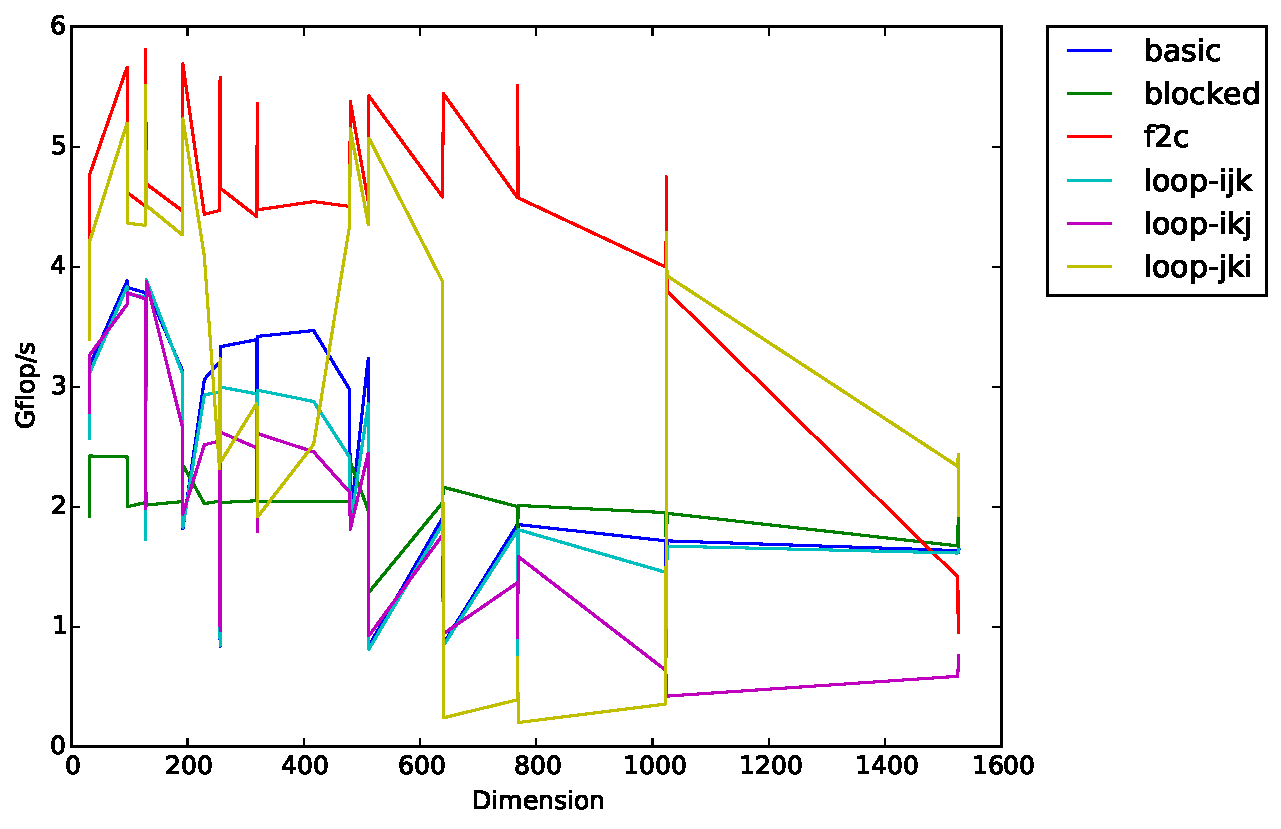
\includegraphics[width=0.7\tw]{fig-opts-inner-results.pdf}

  \caption{\textbf{Performance Comparison of Loop Order Optimizations --}
    We intentionally omit the results for BLAS nad MKL implementations in
    order to focus on the behavior at the performance range of the
    optimization.}

  \label{fig-opts-inner-results}

\end{figure}


As it is clear from the results in Figure~\ref{fig-opts-inner-results},
we achieved significant performance improvement just by changing the
order of loops; thus accessing memory efficiently. We also got an extra
ordinary result between 700-1000 which will be inspected in further
iterations.
\medskip
